%TODO: Talk about how transactions can be composed.
\section{Packet transactions}
\label{s:transactions}

\begin{figure*}[!t]
\begin{minipage}{0.5\textwidth}
\begin{small}
\begin{lstlisting}[style=customc]
#define NUM_FLOWLETS    8000
#define THRESHOLD       5
#define NUM_HOPS        10

struct Packet {
  int sport;
  int dport;
  int new_hop;
  int arrival;
  int next_hop;
  int id; // array index
};

int last_time [NUM_FLOWLETS] = {0};
int saved_hop [NUM_FLOWLETS] = {0};

void flowlet(struct Packet pkt) {
  pkt.new_hop = hash3(pkt.sport,
                      pkt.dport,
                      pkt.arrival)
                % NUM_HOPS;

  pkt.id  = hash2(pkt.sport,
                  pkt.dport)
            % NUM_FLOWLETS;

  if (pkt.arrival - last_time[pkt.id] @\label{line:ifStart}@
      > THRESHOLD)
  { saved_hop[pkt.id] = pkt.new_hop; } @\label{line:ifEnd}@

  last_time[pkt.id] = pkt.arrival;
  pkt.next_hop = saved_hop[pkt.id];
}
\end{lstlisting}
\end{small}
\caption{Flowlet switching written in \pktlanguage}
\label{fig:flowlet_code}
\end{minipage}
%
\vrule\quad
%
\begin{minipage}{0.4\textwidth}
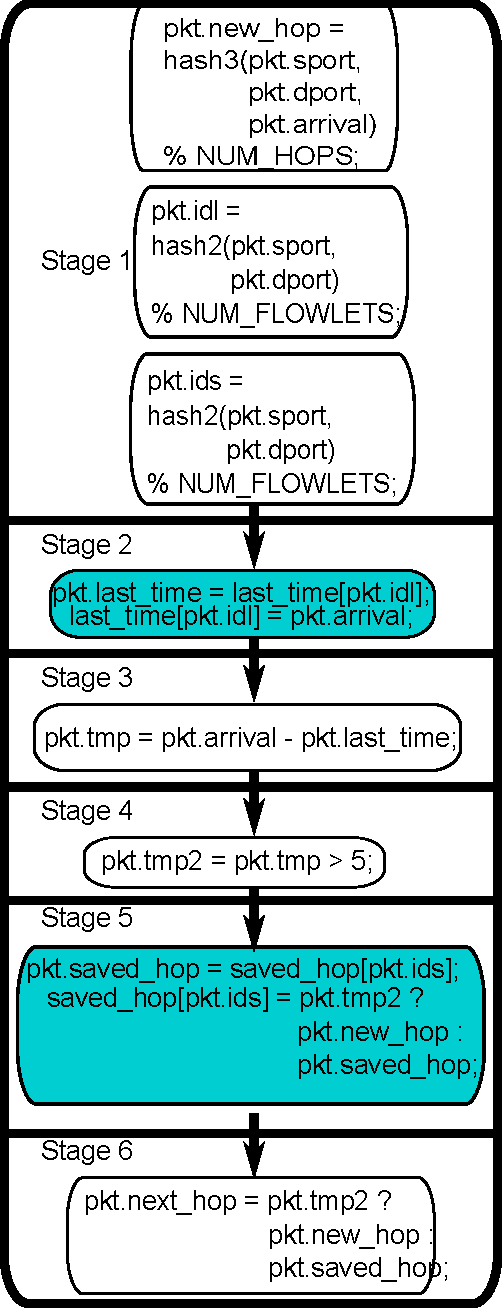
\includegraphics[width=0.8\columnwidth]{pipe.pdf}
\caption{Compiled 6-stage \absmachine pipeline implementing flowlet
switching.  Control flows from top to bottom. Atoms manipulating state are
shaded in blue.}
\label{fig:flowlet_pipeline}
\end{minipage}
\end{figure*}

We now illustrate programming using packet transactions in \pktlanguage, using
flowlet switching~\cite{flowlets} as an example. Flowlet switching is a
load-balancing algorithm that sends bursts of packets (called flowlets) from a
TCP flow on different paths, provided the bursts are separated by a large
enough time interval to ensure packets do not arrive out of order at a TCP
receiver. Figure~\ref{fig:flowlet_code} shows flowlet switching in
\pktlanguage. For simplicity, we hash only the source and destination ports; it
is easy to extend it to the full 5-tuple.

This example demonstrates the core language constructs in \pktlanguage. All
packet processing happens in the context of a packet transaction (the function
\texttt{flowlet} starting at line 17). The function's argument {\tt pkt}
declares the fields in a packet (lines 5--12)\footnote{We use fields to refer
to both packet headers such as source port ({\tt sport}) and destination port
({\tt dport}) and packet metadata ({\tt id}).} that can be referenced by the
function body (lines 18--32).  The function body can also modify persistent
switch state using global variables (e.g.  \texttt{last\_time} and
\texttt{saved\_hop} on lines 14 and 15, respectively).

Conceptually, the switch invokes the packet transaction function on each
incoming packet sequentially. To the programmer, the function modifies the
passed-in packet argument and runs to completion before processing the next
packet.  The function may invoke \textit{intrinsics} such as \texttt{hash2} on
line 23 to use hardware accelerators such as hash generators.  The \pktlanguage
compiler uses an intrinsic's signature to infer dependencies and supplies a
canned run-time implementation, but otherwise does not analyze an intrinsics's
internal behavior.

\subsection{Constraints on the language}
The overall language is a constrained subset of C
(Table~\ref{tab:restrict}).  These constraints are required for
deterministic performance.  Memory allocation, unbounded iteration
counts, and unstructured control flow all cause variable performance,
which may prevent an algorithm from achieving line rate.
Furthermore, all accesses to a given array within one execution of a
transaction, i.e. one packet, must use the same array index. For
example, all read and write accesses to the array \texttt{last\_time}
use the index \texttt{pkt.id}, which is constant for each packet, but
can change between packets. This restriction mirrors restrictions on
memories, where supporting distinct read and write addresses every
clock cycle is challenging.
%TODO: Try and address this.
%\MA{Do we model this restriction in PISA?
%  It would be better to add it to Sec 2.}

\begin{table}
  \begin{tabular}{p{0.9\columnwidth}}
    No iteration (while, for, do-while).\\
    No goto, break, or continue.\\
    No pointers.\\
    No dynamic memory allocation / heap.\\
    Array index is constant for each transaction execution.\\
    No access to data i.e. unparsed portion of the packet.\\
    No arrays in packet fields.\\
  \end{tabular}
  \caption{Restrictions in \pktlanguage}
  \label{tab:restrict}
\end{table}

\subsection{Handling multiple transactions}
\label{ss:multiple}

%TODO: This is very rough as it stands now.
So far, we have discussed how we would express a single packet transaction,
which corresponds to a single data-plane algorithm. In practice, multiple such
data-plane algorithms would run simultaneously on a switch, each on its own
subset of packets. To accommodate multiple transactions, we envision providing
a \textit{guard} for each of these transactions: a packet predicate that
specifies which subset of packets each transaction runs on. This guard could be
placed in the match portion of a match-action pipeline, while the actions
themselves are produced by the result of compiling packet transactions. This
also provides a straightforward mechanism to embed packet transactions into a
standard match-action pipeline. Combining multiple transactions that run on
overlapping subsets of packets requires further work, which we leave for future
work. For the rest of this paper, we focus only on compiling a \textit{single}
packet transaction to a programmable switch.
